
\section{Benchmark Tests}
\label{section: btests}
This section gives insight how the proposed method improves upon methods proposed by existing literature. An improvement is presented with an elaborate example, called a benchmark tests. The benchmark tests, BTests for short include an image of the starting environment, a description of the task, the final knowledge graph and a hypothesis graph which should be generated once the algorithm is implemented. The hypothesis graph may skip certain steps which are not the focus the BTest, and would only clutter the HGraph. \\

Once again the legend for a HGraph is displayed.\\

\begin{figure}[H]
     \centering
     \begin{subfigure}[b]{0.5\textwidth}
         \centering
         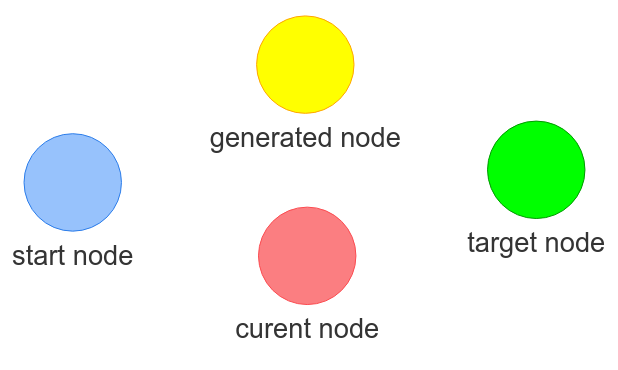
\includegraphics[width=\textwidth]{figures/hgraph_legend_nodes.png}
         \caption{4 nodes used in the HGraph, \textbf{\large Node labels with R:, M: or RM: indicate that the robot is present in the node (R), a model is available (M)}}
     \end{subfigure}
     
     \begin{subfigure}[b]{0.49\textwidth}
         \centering
         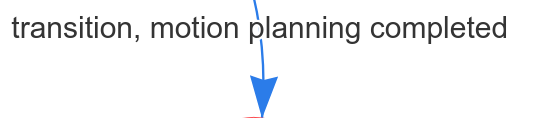
\includegraphics[width=\textwidth]{figures/hgraph_legend_transition1.png}
         \caption{Arrow with solid line}
     \end{subfigure}
    \hfill 
    \begin{subfigure}[b]{0.49\textwidth}
         \centering
         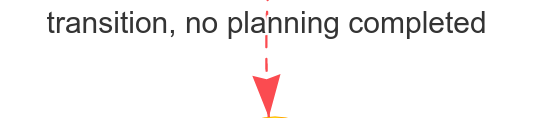
\includegraphics[width=\textwidth]{figures/hgraph_legend_transition2.png}
         \caption{Arrow with dashed line}
     \end{subfigure}
   \caption{HGraph Legend}
    \label{figure: hgraph_legend2}
\end{figure}


\subsection{Blockade by the Duck}
\Cref{figure: blockade_by_duck} displays a robot, 3 unmovable walls, a movable yellow duck and a movable red cube. \textbf{The task} given to the robot is to place the red cube inside the walls. The duck is "guarding" the target location of the red cube. The robot has to first detect, and then to take care of the duck by pushing it to a unspecified location such that the cube can pass through. It is assumed that there is enough space around the objects for system identification, alternatively system identification could be performed on the individual objects, and then perform the blockade by duck task. This BTest already involves many different aspects. Such as system identification on the robot itself, the red cube, the green wall and the duckling, motion planning, manipulation planning and replanning. The goal of this BTest is to give insight that the proposed methods can do all these different aspects.

\begin{figure}[H]
    \centering
    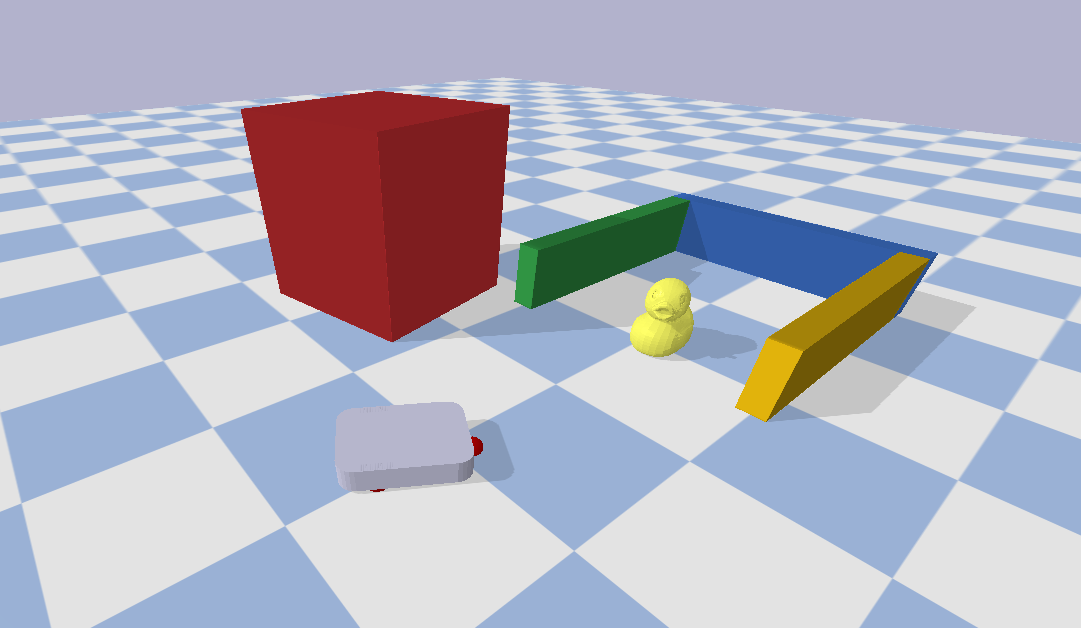
\includegraphics[width=0.6\textwidth]{figures/blockade/blockade_by_duck.png}
    \caption{The robot is tasked with placing the cube inside the walls, only this is guarded by a duckling.}
    \label{figure: blockade_by_duck}
\end{figure}

\begin{figure}[H]
     \centering
     \begin{subfigure}[b]{0.49\textwidth}
         \centering
         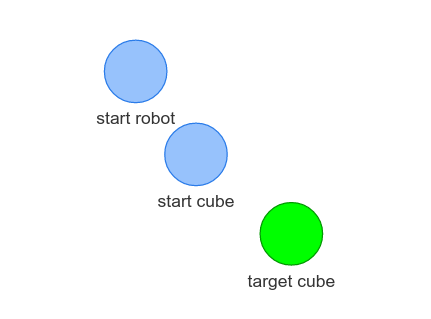
\includegraphics[width=\textwidth]{figures/blockade/1.png}
         \caption{Creating starting and target nodes}
     \end{subfigure}
     \hfill
     \begin{subfigure}[b]{0.49\textwidth}
         \centering
         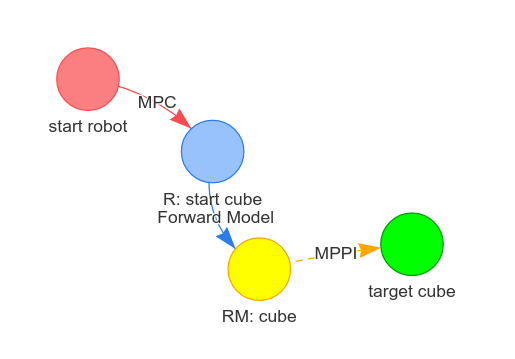
\includegraphics[width=\textwidth]{figures/blockade/2.png}
         \caption{Generate transitions and set start robot as current node}
     \end{subfigure}
     
     \begin{subfigure}[b]{0.49\textwidth}
         \centering
         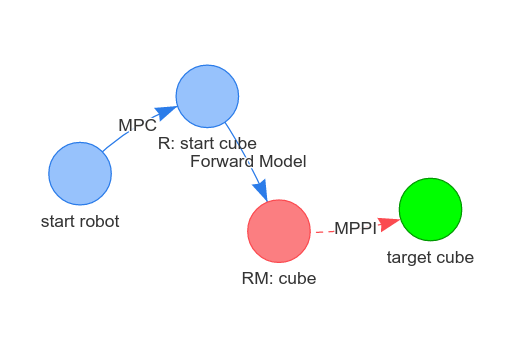
\includegraphics[width=\textwidth]{figures/blockade/3.png}
         \caption{Execute first 2 transitions}
     \end{subfigure}
     \hfill
     \begin{subfigure}[b]{0.49\textwidth}
         \centering
         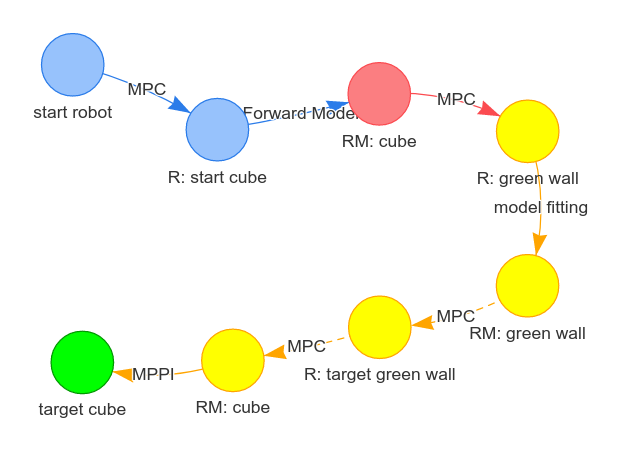
\includegraphics[width=\textwidth]{figures/blockade/4.png}
         \caption{In manipulation a subtask is created to move the green wall, these transitions are expected to complete successfully, completing the task}
     \end{subfigure}
     \caption{HGraph generating hypothesis to push the unmovable green wall and then push the cube to the target position. The figure continues on the next page. For the legend, see \cref{figure: hgraph_legend}}
     \label{figure: blockade_hgraph_first}
\end{figure}

As can be seen in \cref{figure: blockade_hgraph_first}, the HGraph has planned to push the cube toward the target position over the shortest path. On this path the (up to now) unknown green wall stands which needs to be moved before the cube can be pushed toward it's target position. The green wall needs to be pushed such that is does not intersect with the planned path for the cube. \\

The HGraph displayed in \cref{figure: blockade_hgraph_first,figure: blockade_hgraph_second} skips multiple steps in order to focus on the important steps. One of these skipped steps for example is system identification to find a model for the robot itself or the removal of insignificant nodes. 

\begin{figure}[H]
     \centering
     \begin{subfigure}[b]{0.49\textwidth}
         \centering
         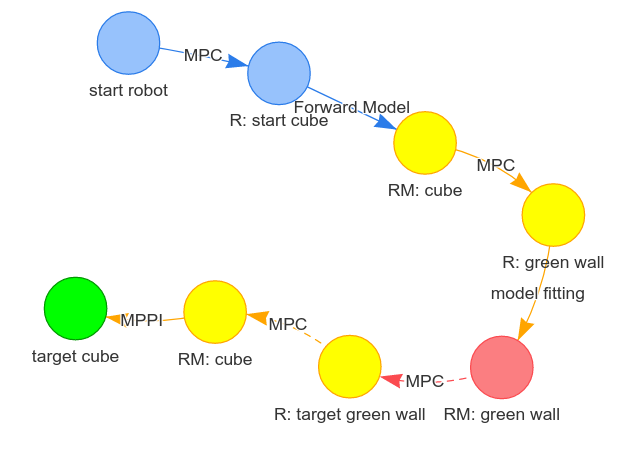
\includegraphics[width=1\textwidth]{figures/blockade/5.png}
         \caption{Robot drives to green wall and performs system identification}
     \end{subfigure}
     \hfill
     \begin{subfigure}[b]{0.49\textwidth}
         \centering
         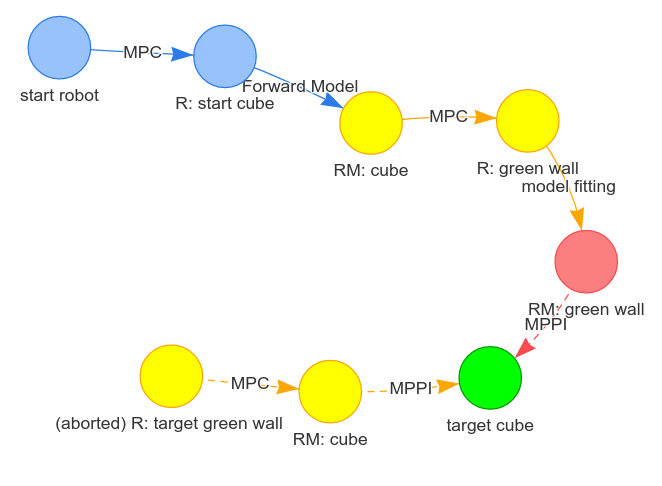
\includegraphics[width=\textwidth]{figures/blockade/6.png}
         \caption{Green wall appears to be unmovable, pushing the green wall is impossible, abort subtask to push green wall to target position}
     \end{subfigure}

     \begin{subfigure}[b]{0.49\textwidth}
         \centering
         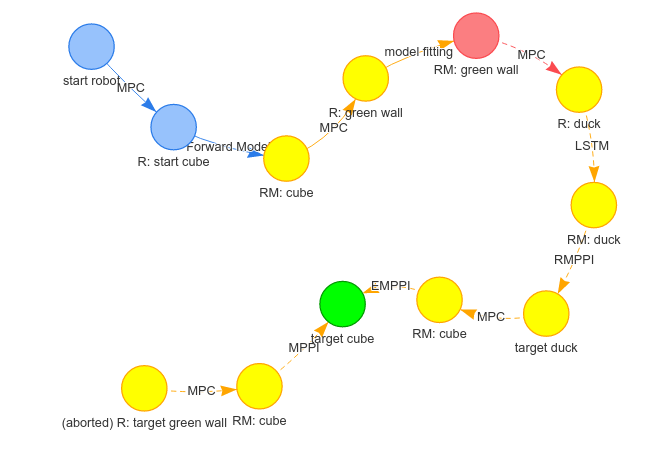
\includegraphics[width=\textwidth]{figures/blockade/7.png}
         \caption{Generate a new starting state since much in the environment has now changed, replan a path from starting to target node}
     \end{subfigure}
     \hfill
     \begin{subfigure}[b]{0.49\textwidth}
         \centering
         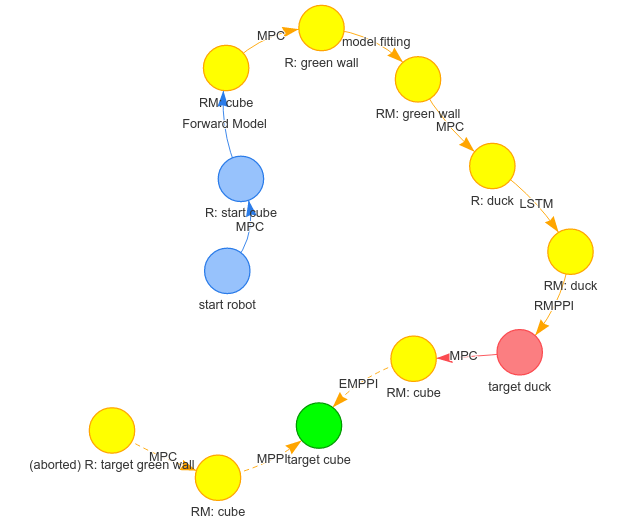
\includegraphics[width=\textwidth]{figures/blockade/8.png}
         \caption{Execute new plan to push the duck and then push the cube to the target position}
     \end{subfigure}
     \caption{HGraph detecting that the green wall is unmovable, generate new hypothesis pushing the movable duck and then push the cube to the target position, For the legend, see \cref{figure: hgraph_legend2}}
     \label{figure: blockade_hgraph_second}
\end{figure}

The proposed approach and expected HGraph tackles a problem which \cite{siciliano_path_2009,wang_affordance-based_2020,scholz_navigation_2016} are not able to solve because they lack a crucial component. \cite{siciliano_path_2009} can navigate through movable obstacles and place objects on target positions. It is however provided with a set of movable and unmovable obstacles, the lack of learning dynamics prevents adaptation to new or changed environments. \cite{wang_affordance-based_2020} is able to navigate among movable obstacles and where required, identify if an object is pushable and if so, push an object to free it's path. A push to free the path is quite different from pushing to a target position. Lacking is thus the ability to manipulate objects to target positions, which is required in the blockade by duck task. The same argument holds for \cite{scholz_navigation_2016} who can navigate and move an object to free the path, but is unable to manipulate an object toward a target position. \\

\begin{figure}[H]
    \centering
    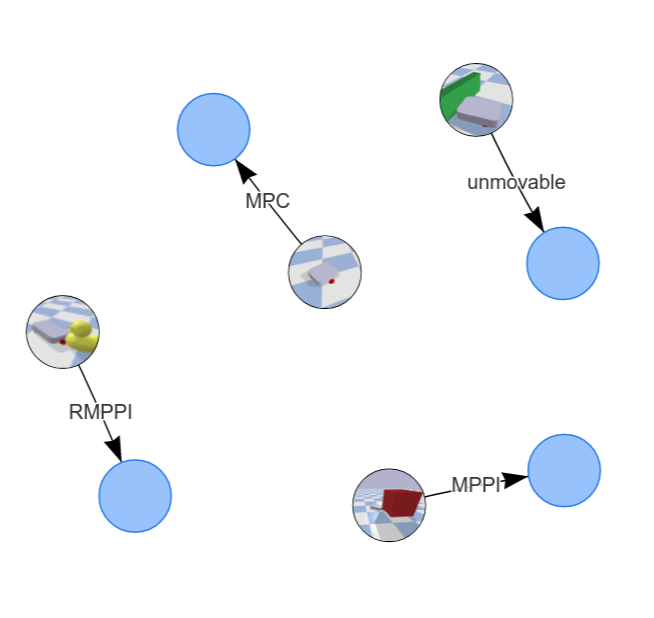
\includegraphics[width=0.6\textwidth]{figures/blockade/blockade_kgraph.png}
    \caption{Knowledge graph after completion of the blockade task.}
    \label{figure: blockade_kgraph}
\end{figure}

\subsection{Surrounded by Cubes}
\Cref{figure: surrounded_by_boxes} displays a robot and 6 cubes, only the green cube is movable, the red, blue and yellow cubes are unmovable. \textbf{The task} given to the robot is to go toward a target location outside of the surrounding boxes. It is assumed that to drive toward target location the robot has to move a cube, moving the red cube gives the shortest path toward the target position, moving the blue cube gives a longer shortest path and moving the green cube gives an even longer shortest path. The goal of this BTest is to show that learned knowledge is stored and makes a difference when encountering objects for the second time. 

\begin{figure}[H]
    \centering
    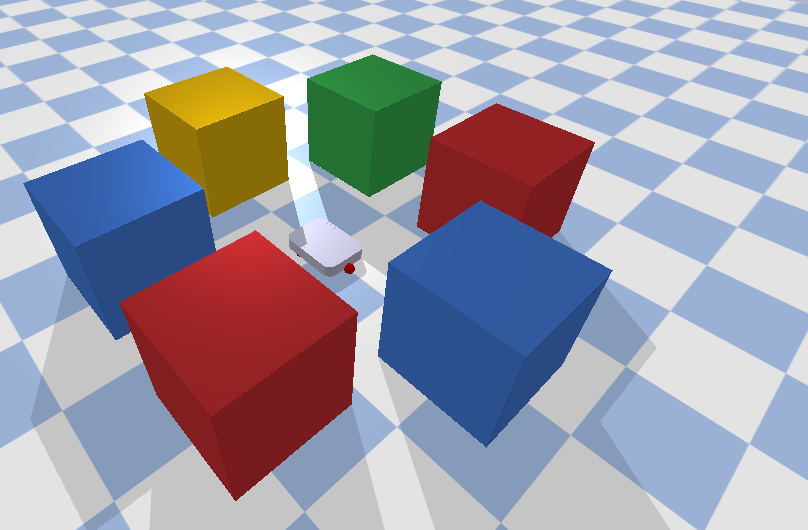
\includegraphics[width=0.6\textwidth]{figures/surrounded/surrounded_by_boxes.png}
    \caption{The robot is tasked with going to a target position outside the surrounding boxes, only one box is movable}
    \label{figure: surrounded_by_boxes}
\end{figure}

\begin{figure}[H]
     \centering
     \begin{subfigure}[b]{0.49\textwidth}
         \centering
         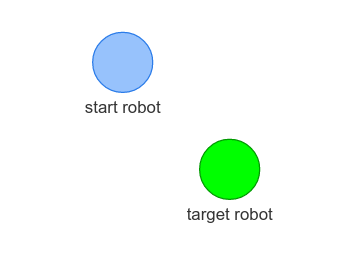
\includegraphics[width=\textwidth]{figures/surrounded/1.png}
         \caption{Creating starting and target node}
     \end{subfigure}
     \hfill
     \begin{subfigure}[b]{0.49\textwidth}
         \centering
         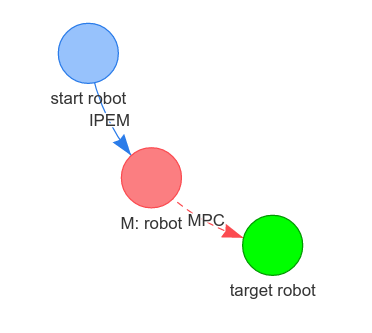
\includegraphics[width=\textwidth]{figures/surrounded/2.png}
         \caption{Generate hypothesis driving toward target position and perform system identification on robot}
     \end{subfigure}
     
     \begin{subfigure}[b]{0.49\textwidth}
         \centering
         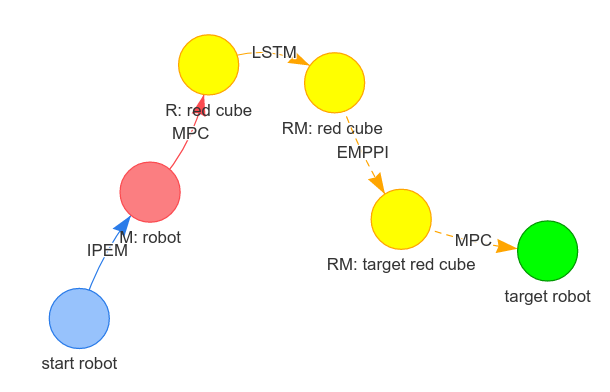
\includegraphics[width=\textwidth]{figures/surrounded/3.png}
         \caption{Find red cube blocking the path which needs to be moved}
     \end{subfigure}
     \hfill
     \begin{subfigure}[b]{0.49\textwidth}
         \centering
         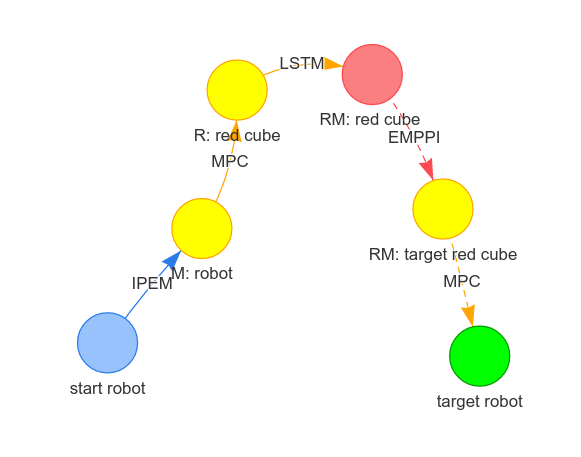
\includegraphics[width=\textwidth]{figures/surrounded/4.png}
         \caption{Drive toward red cube and perform system identification}
     \end{subfigure}
     \begin{subfigure}[b]{0.49\textwidth}
         \centering
         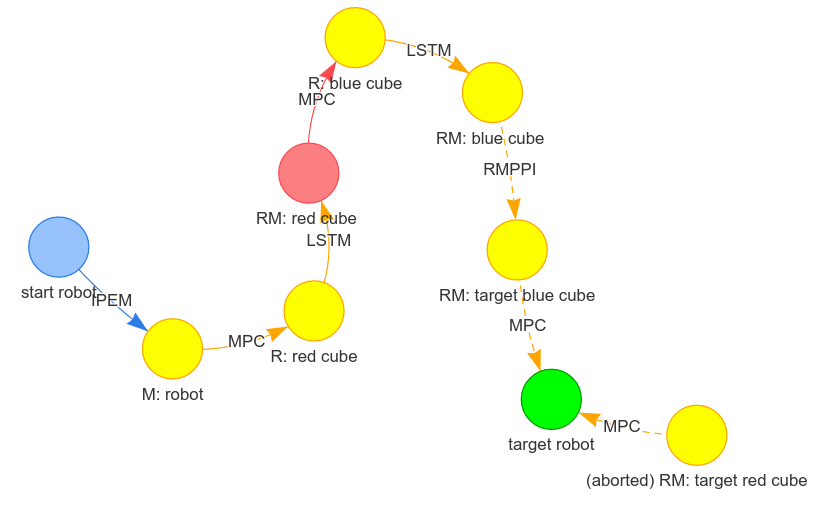
\includegraphics[width=1\textwidth]{figures/surrounded/5.png}
         \caption{The red cube in unmovable, abort subtask and replan to move the blue cube}
     \end{subfigure}
     \hfill
     \begin{subfigure}[b]{0.49\textwidth}
         \centering
         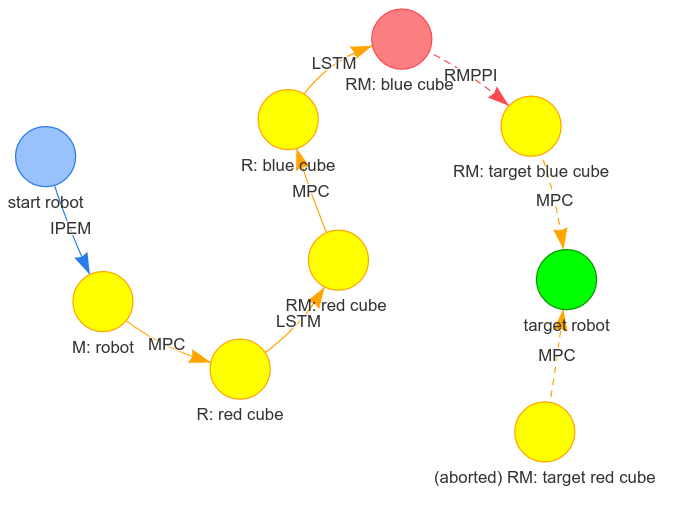
\includegraphics[width=\textwidth]{figures/surrounded/6.png}
         \caption{Drive toward blue cube and perform system identification}
     \end{subfigure}
     \caption{Figure continues on the next page}
\end{figure}

\begin{figure}[H]
    \ContinuedFloat
     \begin{subfigure}[b]{0.49\textwidth}
         \centering
         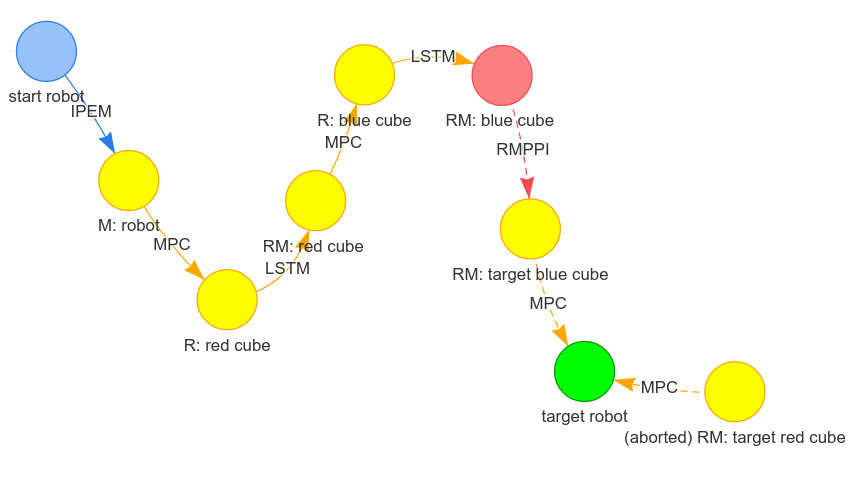
\includegraphics[width=\textwidth]{figures/surrounded/7.png}
         \caption{Blue cube is unmovable, abort subtask and replan to move the green cube}
     \end{subfigure}
     \hfill
     \begin{subfigure}[b]{0.49\textwidth}
         \centering
         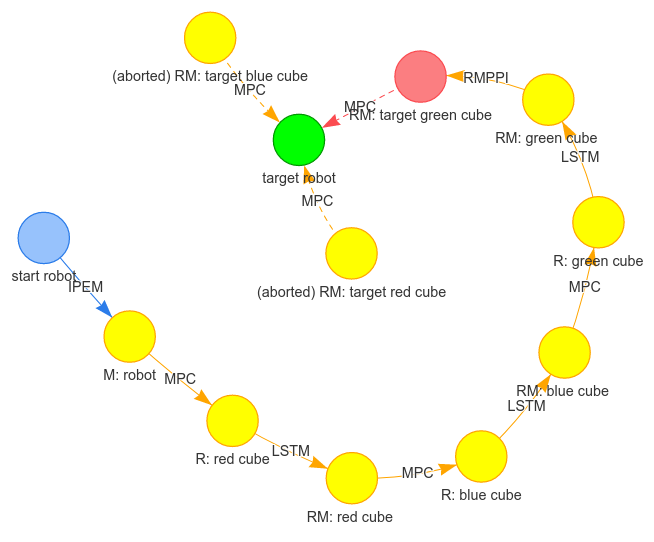
\includegraphics[width=\textwidth]{figures/surrounded/8.png}
         \caption{Green cube is movable, after system identification push it. Now the path is free to drive toward the robot's target position}
     \end{subfigure}
     \caption{After multiple failed hypothesis, a succeeding hypothesis is found which completes the task. For the legend, see \cref{figure: hgraph_legend2}.}
     \label{figure: surrounded_hgraph_second}
\end{figure}

\begin{figure}[H]
    \centering
    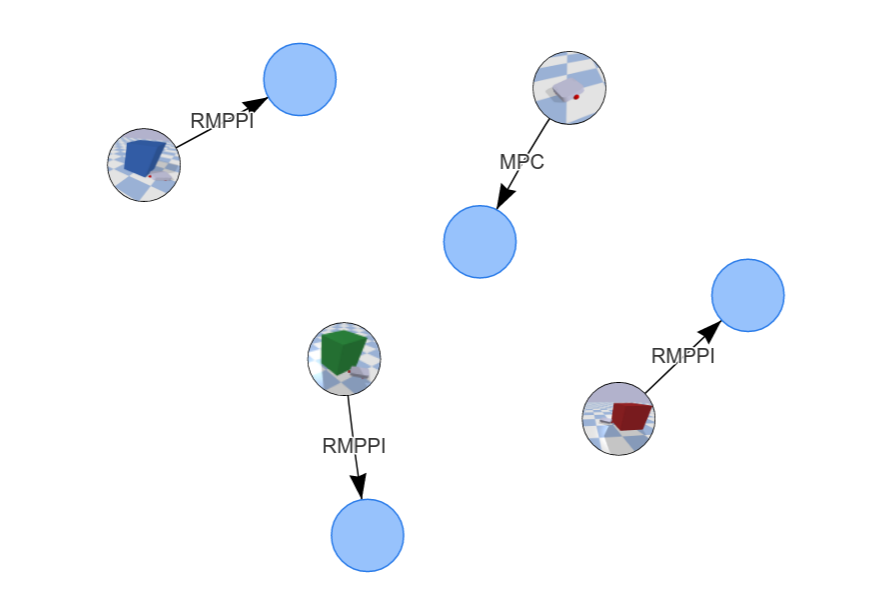
\includegraphics[width=0.7\textwidth]{figures/surrounded/surrounded_kgraph.png}
    \caption{Knowledge graph after completion of the surrounded task.}
    \label{figure:  surrounded_kgraph}
\end{figure}

\begin{figure}[H]
    \centering
    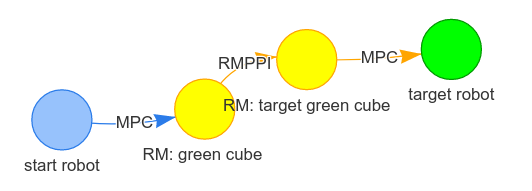
\includegraphics[width=0.5\textwidth]{figures/surrounded/thank_you_hgraph.png}
    \caption{The hypothesis graph after redoing the same surrounded task for the second time. For the legend, see \cref{figure: hgraph_legend2}.}
    \label{figure: surrounded_with_prior_knowledge}
\end{figure}

The second time the same surrounded task given to the robot some crucial knowledge is captured by the knowledge graph. Prior knowledge about the movability of the red, blue and green cubes is provided and system models for the cubes an the robot. as can be seen in \cref{figure: surrounded_with_prior_knowledge} immediately goes for pushing the movable cube to then drive toward the target position.

\subsection{Swapping Objects}
\Cref{figure: swap_hgraph} displays a robot and movable obstacles. \textbf{The task} given to the robot is to swap the two objects, the duck must go to the position where the cube currently is and vise versa. The goal of this BTest is to give insight into the proposed methods ability to handle multiple objects, and to show that hierarchical methods yields a suboptimal solution. \\

\begin{figure}[H]
    \centering
    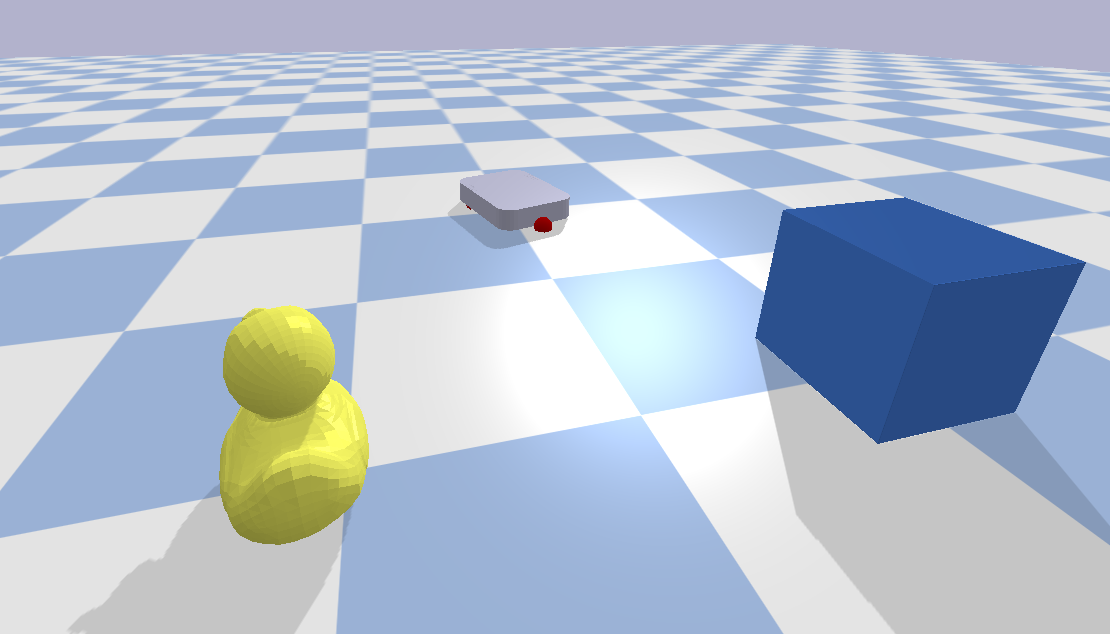
\includegraphics[width=0.6\textwidth]{figures/swap/swap_obstacles.png}
    \caption{The robot is tasked with swapping the two obstacles}
    \label{figure: swap_obstacles}
\end{figure}

\begin{figure}[H]
     \centering
     \begin{subfigure}[b]{0.49\textwidth}
         \centering
         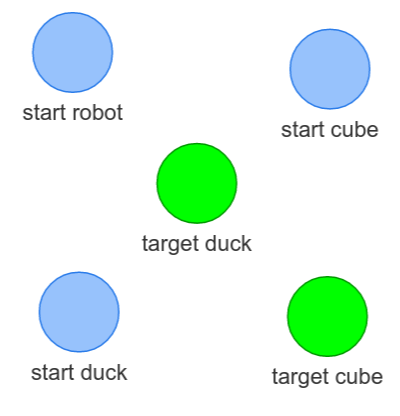
\includegraphics[width=\textwidth]{figures/swap/1.png}
         \caption{Creating starting and target nodes}
     \end{subfigure}
     \hfill
     \begin{subfigure}[b]{0.49\textwidth}
         \centering
         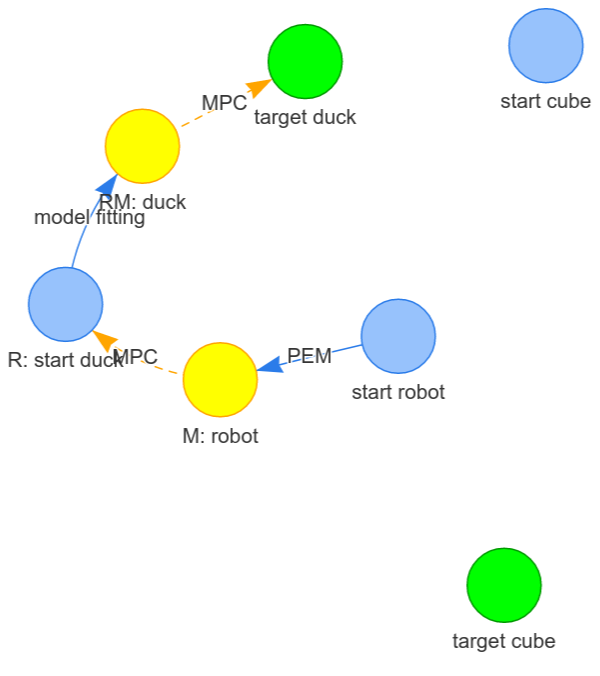
\includegraphics[width=\textwidth]{figures/swap/2.png}
         \caption{Generate hypothesis to perform system identification on duck and place duck on target position}
     \end{subfigure}
     \caption{Figure continues on the next page}
\end{figure}

\begin{figure}[H]
    \ContinuedFloat
     \begin{subfigure}[b]{0.49\textwidth}
         \centering
         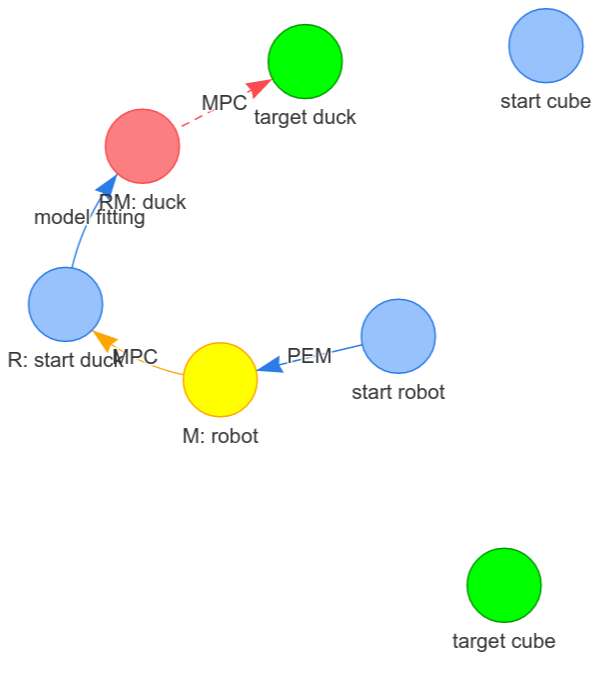
\includegraphics[width=\textwidth]{figures/swap/3.png}
         \caption{Execute first 3 transitions}
     \end{subfigure}
     \hfill
     \begin{subfigure}[b]{0.49\textwidth}
         \centering
         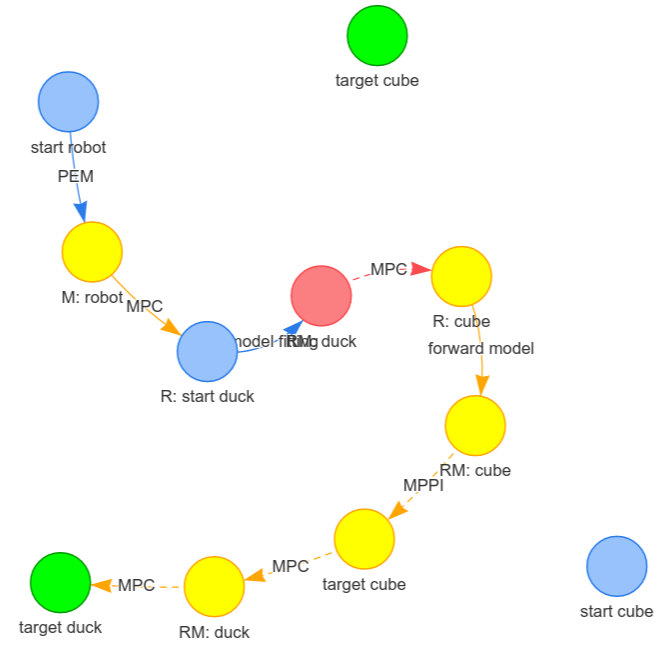
\includegraphics[width=\textwidth]{figures/swap/4.png}
         \caption{The cube is a obstacle which needs to be moved during planning the duck to target position}
   \end{subfigure}
   
    \begin{subfigure}[b]{0.49\textwidth}
         \centering
         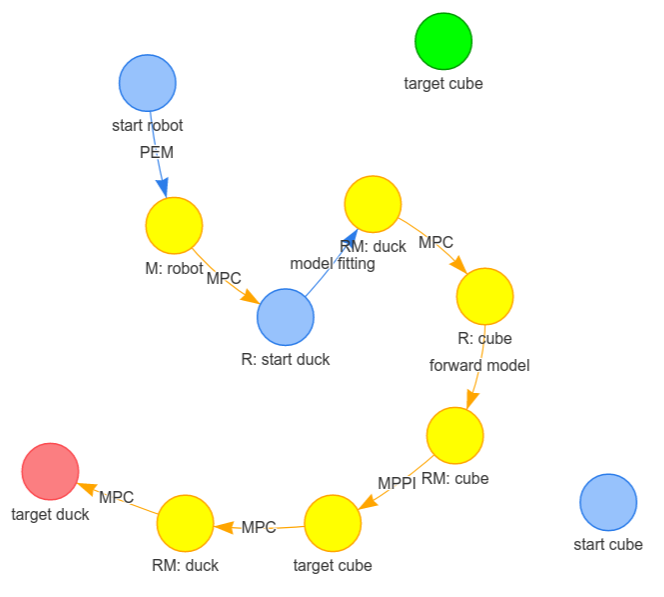
\includegraphics[width=\textwidth]{figures/swap/5.png}
         \caption{Execute transitions up until placing the duck on the target position}
     \end{subfigure}
     \hfill
     \begin{subfigure}[b]{0.49\textwidth}
         \centering
         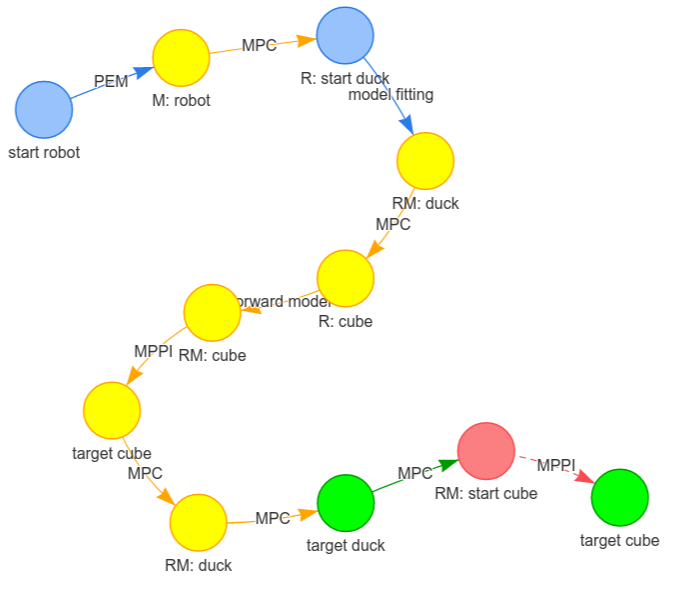
\includegraphics[width=\textwidth]{figures/swap/6.png}
         \caption{Create hypothesis to place cube on target position and drive toward cube}
     \end{subfigure}
     \caption{Swapping two objects, for the legend, see \cref{figure: hgraph_legend2}.}
     \label{figure: swap_hgraph}
\end{figure}

\begin{figure}[H]
    \centering
    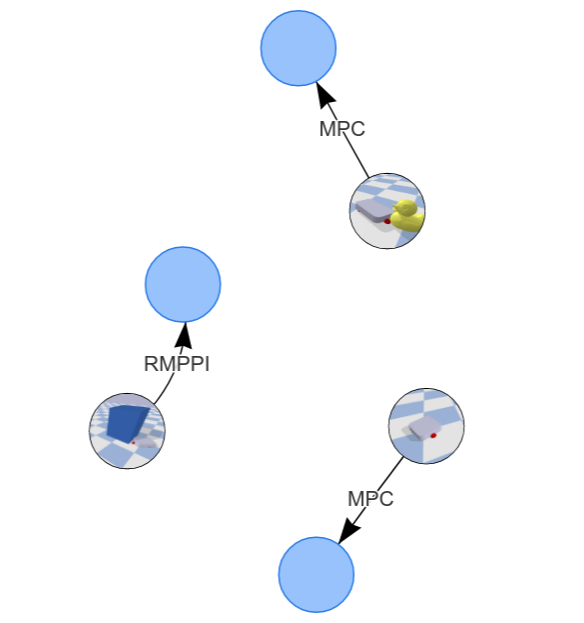
\includegraphics[width=0.6\textwidth]{figures/swap/swap_kgraph.png}
    \caption{Knowledge graph after completion of the swap task.}
    \label{figure: swap_kgraph}
\end{figure}

The expected HGraph shows promising results, the ability to handle multiple objects of which the start and target positions are overlapping. Whilst object rearrangement algorithms exists \cite{krontiris_dealing_2015}, only \cite{sabbagh_novin_model_2021} implements target positions of environment objects, it however only considers a single object and a free path. Allowing to conclude that learning object dynamics \textit{and} \ac{NAMO} \textit{and} specifying objects target positions is a fairly new area of robotics. \\

A limitation due to the hierarchical search in the HGraph becomes visible. Imagine the objects to be swapped are very far apart. The proposed solution drives (possibly whilst being closer to the cube) to the starting position of the duck then to the cube, moves the cube a bit, back to the duck, then push the duck to target position and finally push cube to target position. Worst case, the robot is driving the distance between both starting positions 5 times, optimal is less than 3 times (assuming the robot is less than the initial cube-duck distance from either the duck or the cube). \cite{goldberg_asymptotically_2020} already emphasised the suboptimality of hierarchical solutions. In addition, model mismatch and failure to find the existing path during motion and manipulation planning decrease the optimality of the plan found by the proposed method. Suboptimality is acceptable since that is not the goal of the literature study.





